\chapter{ACL.Test.Suite}
\section{AUnit}
AUnit 3.5 is a test framework based on a set of Ada packages. In our
project it's intended to run the unit tests to verify correctness of
the source code. AUnit 3.5 can be downloaded in
LIBRE\footnote{http://libre.adacore.com/tools/aunit/}. Some video
tutorials of AUnit by Daniel Bigelow are also provided. The user
manual named AUnit
Cookbook\footnote{http://docs.adacore.com/aunit-docs/aunit.html} can
be used for a deeper understanding.

To use the AUnit library in our project we should first include the head data:
\begin{lstlisting}
  with AUnit.Assertions;
\end{lstlisting}

The common structure of AUnit is described in Figure \ref{TestAunit}:
\begin{figure}[htp]
  \centering
  \includegraphics[scale=0.7]{Pictures/Structure_Test.pdf}
  \caption{The structure of tests in AUnit.}\label{TestAunit}
\end{figure}

Usually one test case is for one condition, but there can be many test
cases for one operation. For instance, we want to test the basic
operations in \texttt{Crypto.Types.Big\_Number} file, then we have
e.g. Test-Case-A for addition and Test-Case-B for subtraction etc.. A
test suite collects these test cases. On the other hand the test suite
is controlled by a test runner. All test cases are in a queue waiting
to execute. This is the general workflow of AUnit. We use it in the
ACL to make the regression tests.

Test cases for one target operation are all registered through
procedure called \texttt{Register\_\-Tests}. It returns detailed
informations by entering the procedure and occuring of errors, where
the error is and additionally the test case number.
\begin{lstlisting}
  procedure Register_Tests(T : in out Template_Test) is
    use Test_Cases.Registration;
  begin
    Register_Routine(T, Template_Test1'Access,"Template");
  end Register_Tests;
\end{lstlisting}\\ \ \\
Furthermore all test cases have a namer procedure, which returns the prefix name of the test cases. The registered name in the following procedure is the prefix name, it will be showed in front of all test cases in this procedure.
\begin{lstlisting}
  function Name(T : Template_Test) return String_Access is
  begin
	return new String'("Template Test");
  end Name;
\end{lstlisting}\\ \ \\
A template test example:
\begin{lstlisting}
  procedure Template_T(T: in out Test_Cases.Test_Case'Class) is
    use AUnit.Assertions; 
  begin      
    Assert(A = B, "Failed with A and B.");
  end Template_T;
\end{lstlisting}
If the result against the expectation, in other words, A is unequal B, then an error message will be showed. And so is the name of the test case and the name of the procedure. At the same time the test case number is also included in the error message.

\section{GCOV}
GCOV is a test coverage program, it helps us discover untested parts of our program. After calling GCOV it shows the performance of our test cases, i.e. which code fragments are covered by the test cases. GCOV works best with a programming style that places only one statement on each line, that is, code without optimization.

GCOV should be run with the current directory the same as that when you invoked the compiler. The data should be compiled with \lstinline[style=BashInputStyle]´make gcov´,
then, an accompanying \texttt{.gcov} file will be placed in the object file directory.  
Each \texttt{.gcov} file is produced for each source file containing code, which was compiled to produce the data files. In the \texttt{.gcov} files unexecuted lines are marked with '$\#\#\#\#$'. The execution count of '-' is for lines containing no code. The execution counts are cumulative. If the program is executed again without removing the files, the count for the number of times in each line would be added to the results of the previous runs. 
The output would be as following:\\
\hspace*{1cm}\texttt{File 'test-sha1.ads'}\\
\hspace*{1cm}\texttt{Lines executed:100.00\% of 3}\\
\hspace*{1cm}\texttt{test-sha1.ads:creating 'test-sha1.ads.gcov'}\\
\\
\hspace*{1cm}\texttt{File '../src/crypto-asymmetric-rsa.ads'}\\
\hspace*{1cm}\texttt{Lines executed:100.00\% of 8}\\
\hspace*{1cm}\texttt{../src/crypto-asymmetric-rsa.ads:creating 'crypto-asymmetric-rsa.ad\-s.gcov'}\\
\\
\hspace*{1cm}\texttt{File '../src/crypto-asymmetric-rsa.adb'}\\
\hspace*{1cm}\texttt{Lines executed:65.36\% of 179}\\
\hspace*{1cm}\texttt{../src/crypto-asymmetric-rsa.adb:creating 'crypto-asymmetric-rsa.ad\-b.gcov'}\\

The first line shows the executed file name, the second line is the percent coverage of the data. The last line tells us that the logfile is produced by GCOV. A logfile may have the following format:
\begin{lstlisting} 
14:   70:   procedure Set_Most_Significant_Bit
                      (X: in out Big_Unsigned) is
 -:   71:   begin
14:   72:      X.Last_Index := Max_Length;
14:   73:      X.Number(Max_Length) := X.Number(Max_Length) or
 -:   74:        Shift_Left(Mod_Type(1), Mod_Type'Size-1);
14:   75:   end Set_Most_Significant_Bit; 
	         pragma Inline(Set_Most_Significant_Bit);
\end{lstlisting}
The first number means the execution frequency and the second number is the code number in the original source code. The document in {\tt http://gcc.gnu.org/onlinedocs/gcc/Gc\-ov.html} can be used for further information.
%%%%%%%%%%%%%%%%%%%%%%%%%%%%%%%%%%%%%%%%%%%%%%%%%%%%%%%%%%%%5
%%%%%%%%%%%%%%%%%%%%%%%%%%%%%%%%%%%%%%%%%%%%%%%%%%%%%%%%%%%%%%
\section{LCOV}
LCOV is a graphical front-end for GCOV. It collects gcov data and creates HTML pages containing the source code annotated with coverage information. It also supports easy navigation within the file structure. LCOV can be used for statement, function and branch coverage measurement.
After executing \lstinline[style=BashInputStyle]´make lcov´, 
one file containing all HTML pages will be produced. The current test coverage of the ACL is shown in Figure \ref{LCOVS}, which reaches 90.9\%. The coverage of each file is shown by bars in three colors: red (low $<$ 75\%), (medium $>=$ 75\%) and green (high $>=$ 90\%). The aim of the next step is to achieve the line coverage of at least 95\% for each file.

\begin{figure}[h]
  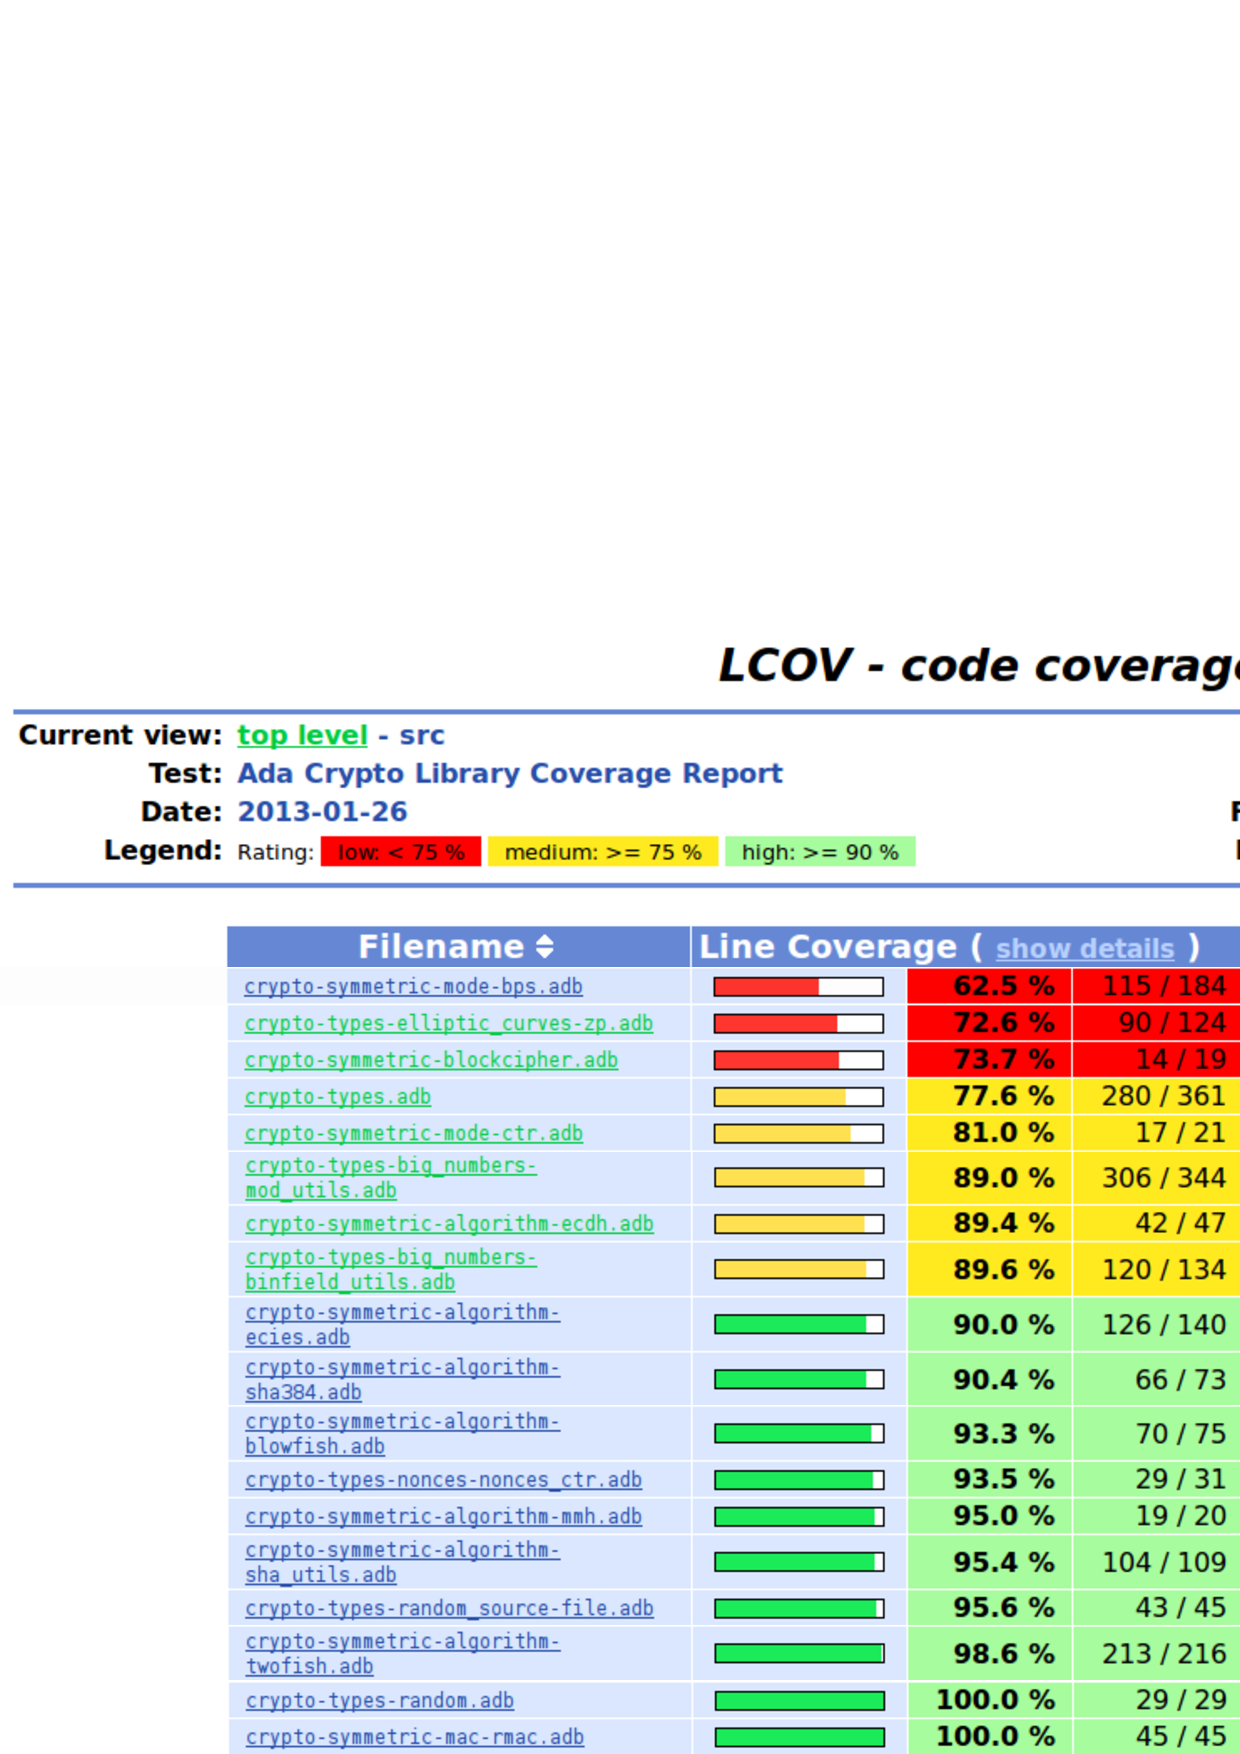
\includegraphics[scale=0.4]{Pictures/LCOV2.pdf} 
  \caption{The current test coverage of the ACL.}\label{LCOVS}
\end{figure}
